\documentclass{beamer}

%------------------------------------------------
% Packages & Fonts
%------------------------------------------------
\usepackage[utf8]{inputenc}
\usepackage{graphicx}
\usepackage{xcolor}
\usepackage{tikz}
\usepackage{lmodern}
\usepackage{amsmath}
\usepackage{booktabs}
\usepackage{multirow}
\usepackage{appendixnumberbeamer}

%------------------------------------------------
% Stanford Colors
%------------------------------------------------
\definecolor{stanfordred}{HTML}{8C1515}
\definecolor{customlightgray}{rgb}{0.9,0.9,0.9}

%------------------------------------------------
% Theme & Color Overrides
%------------------------------------------------
\usetheme{Dresden}

\setbeamercolor{structure}{fg=stanfordred}
\setbeamercolor{title}{fg=stanfordred}
\setbeamercolor{frametitle}{bg=stanfordred, fg=white}
\setbeamercolor{itemize item}{fg=stanfordred}
\setbeamercolor{section in toc}{fg=stanfordred}
\setbeamertemplate{caption}[numbered]

\setbeamercolor{section in head/foot}{bg=customlightgray, fg=stanfordred}
\setbeamerfont{section in head/foot}{size=\scriptsize}
\setbeamertemplate{navigation symbols}{}

%------------------------------------------------
% Custom Footline: only frame number
%------------------------------------------------
\setbeamertemplate{footline}{%
  \leavevmode%
  \hbox{%
    \hspace*{0.85\paperwidth}%
    \begin{beamercolorbox}[wd=0.15\paperwidth,ht=2.5ex,dp=1ex,right]{date in head/foot}%
      \insertframenumber{} / \inserttotalframenumber%
    \end{beamercolorbox}%
  }%
}

\setbeamerfont{frametitle}{size=\small}

%------------------------------------------------
% Document Info
%------------------------------------------------
\title{Local Nonlinear Projection-Based Reduced-Order Models}

\author{%
Sebastian Ares de Parga\textsuperscript{3}, \
Radek Tezaur\textsuperscript{1}, \
Charbel Farhat\textsuperscript{1,2} \
}

\institute{%
  \inst{1} Department of Aeronautics and Astronautics\\
  \inst{2} Institute for Computational and Mathematical Engineering\\
  Stanford University, Stanford, CA 94305, USA\\[0.5ex]
  \inst{3} CIMNE, Barcelona 08034, Spain\\[0.5ex]
}

\date{\today}

\begin{document}

\begin{frame}
  \titlepage
\end{frame}

\begin{frame}{Setup for Paper Campaign}
\small
\textbf{Problem:} 2D Burgers, mesh $250\times250$.

\vspace{0.3em}
\textbf{Test points:}
\[
\boldsymbol\mu_1=(4.56,0.019),\quad
\boldsymbol\mu_2=(4.75,0.020),\quad
\boldsymbol\mu_3=(5.19,0.026).
\]

\vspace{0.2em}
\textbf{Methods included:}
\begin{itemize}
\item Global HPROM (linear POD)
\item Global HQPROM (quadratic manifold)
\item Global HPROM-GPR
\item Local HPROM
\item Local HQPROM
\item Local HPROM-GPR
\end{itemize}
\end{frame}

\begin{frame}{Parameter Domain and Test Points}
\centering
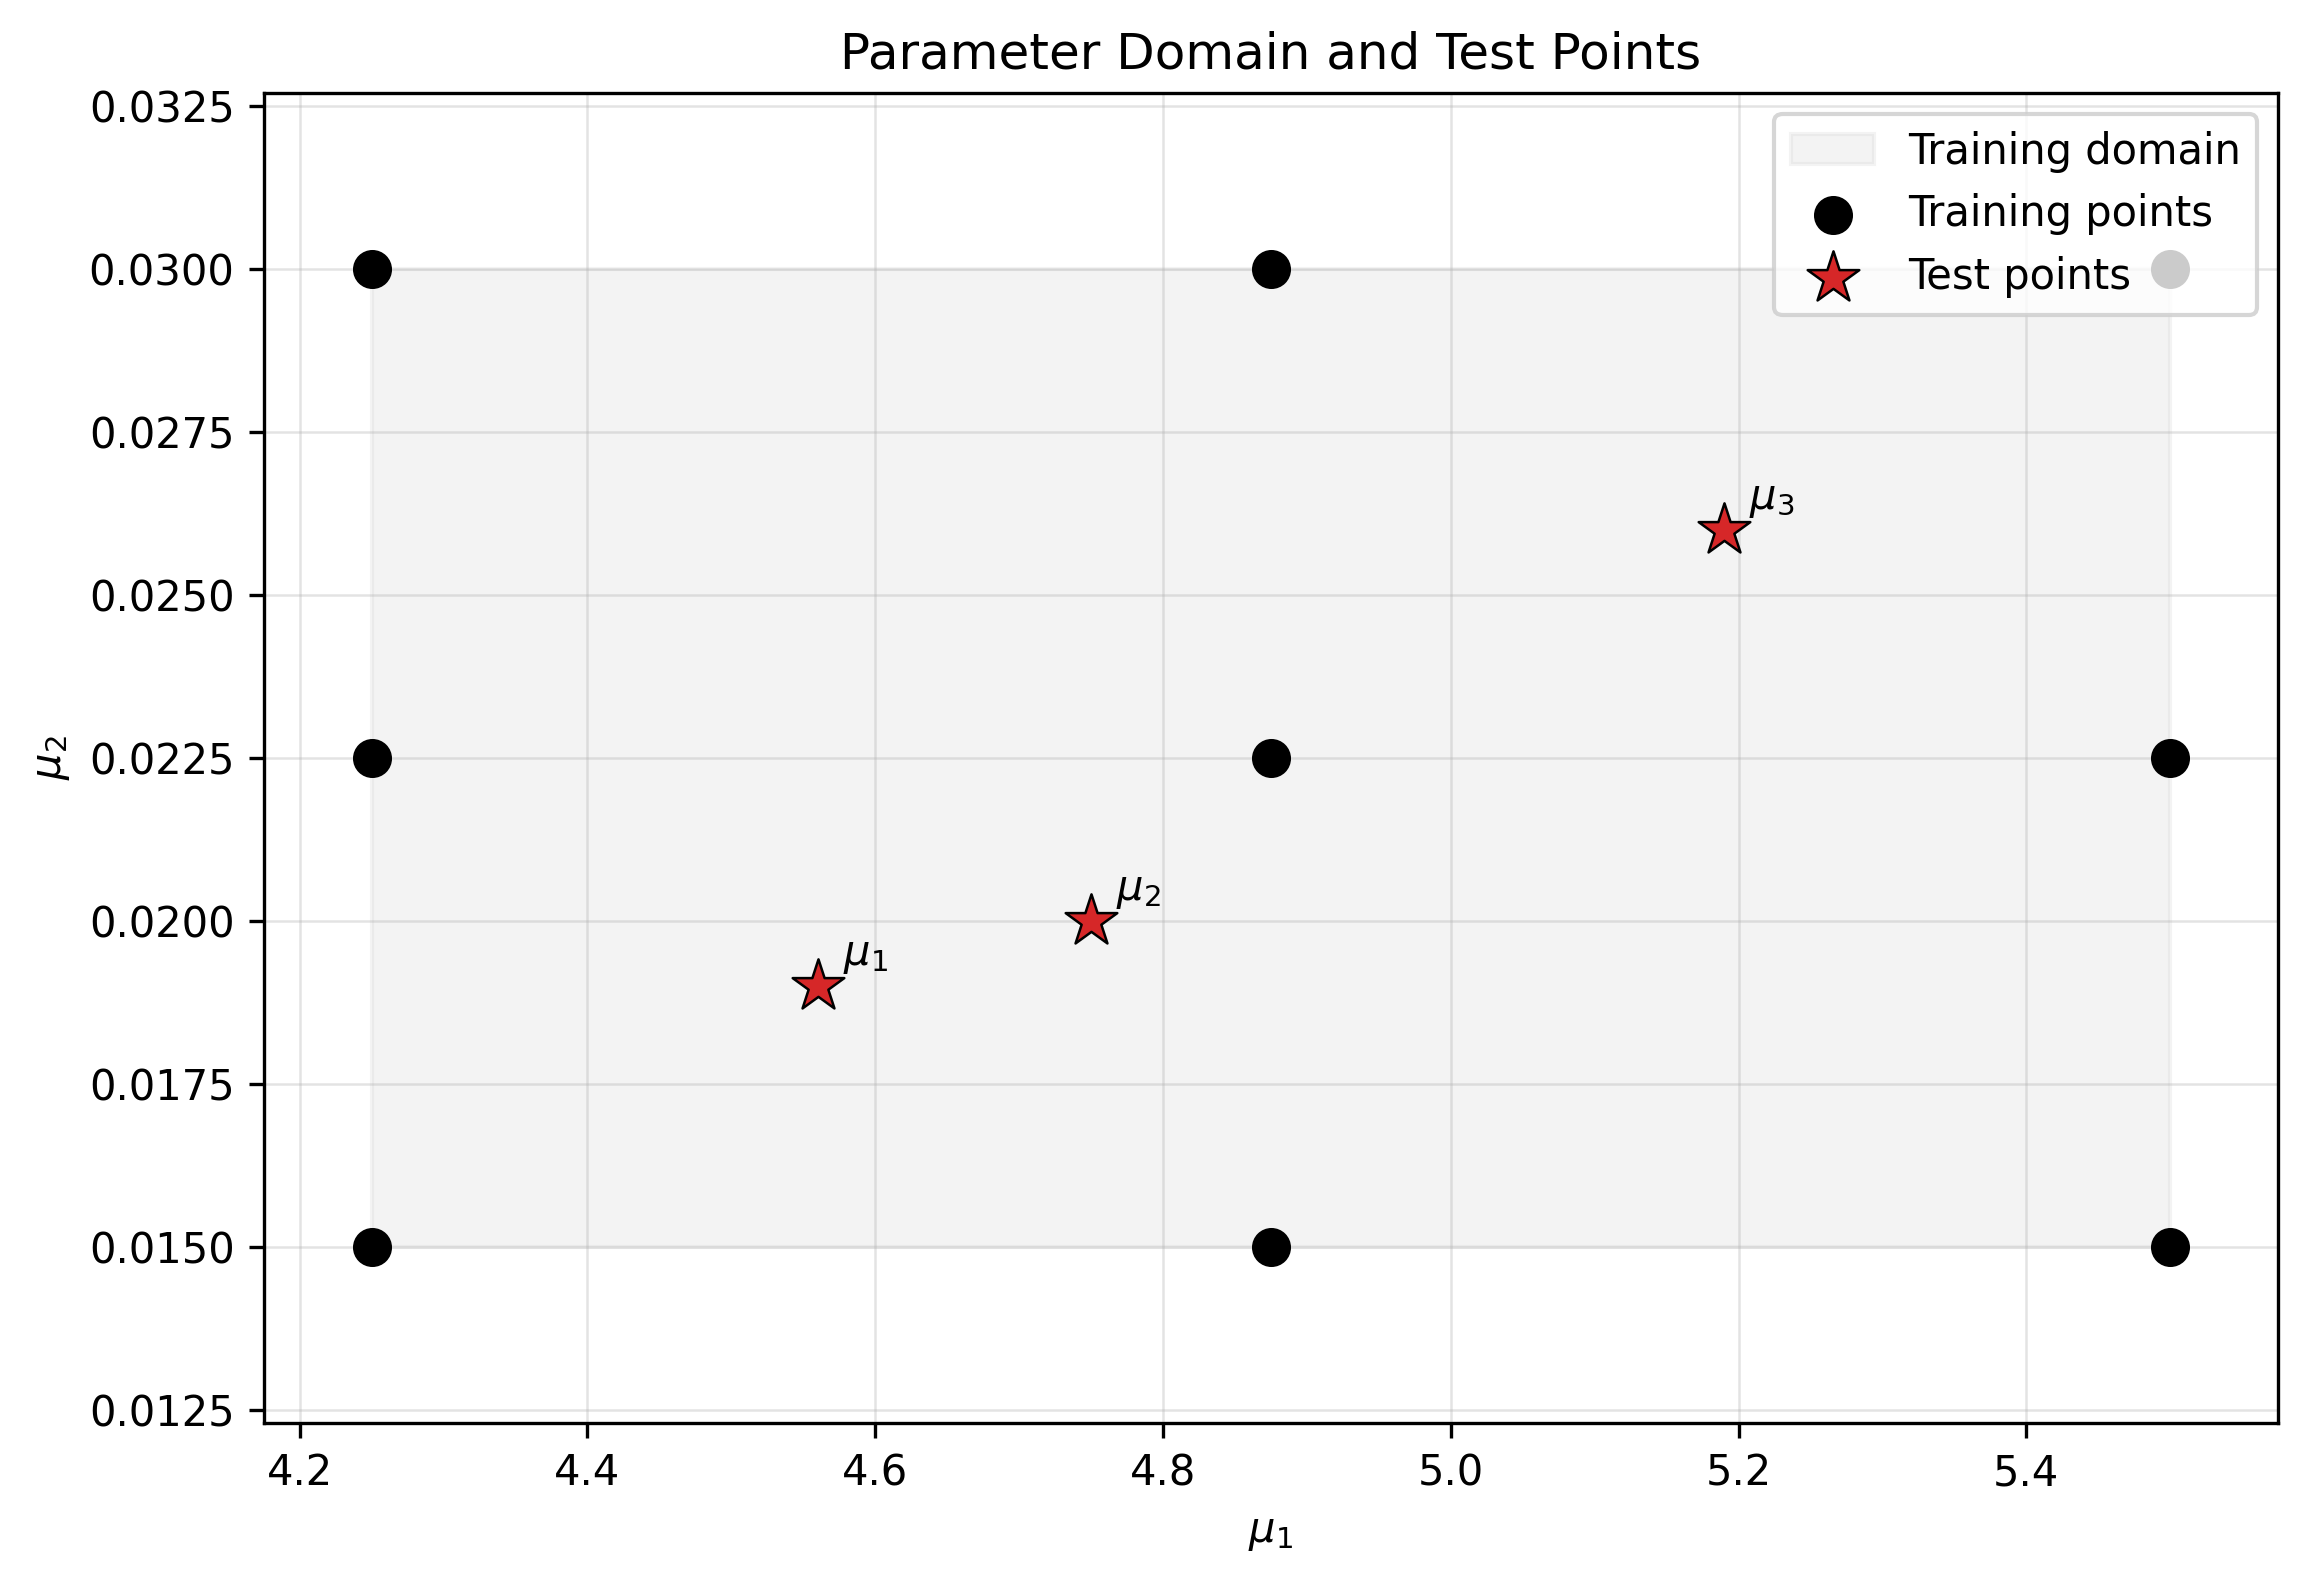
\includegraphics[width=0.82\textwidth]{Figures/parameter_domain_and_test_points.png}
\end{frame}

\begin{frame}{Global ROM Storyline: LSPG + Gauss-Newton}
\small
Given the implicit HDM residual $\mathbf{r}(\mathbf{u})=\mathbf{0}$, define a manifold
\[
\mathbf{u}\approx \mathbf{u}_{\mathrm{ref}}+\widetilde{\mathbf{u}}(\mathbf{q}).
\]
LSPG solves at each time step:
\[
\mathbf{q}^{\star}
=\arg\min_{\mathbf{q}}\;
\frac{1}{2}\left\|\mathbf{r}\!\left(\mathbf{u}_{\mathrm{ref}}+\widetilde{\mathbf{u}}(\mathbf{q})\right)\right\|_2^2.
\]
With Gauss-Newton (current iterate $\mathbf{q}^{(k)}$), the increment $\Delta\mathbf{q}$ is obtained from
\[
\left(\mathbf{\Psi}^{T}\mathbf{J}^{T}\mathbf{J}\mathbf{\Psi}\right)\Delta\mathbf{q}
=-\mathbf{\Psi}^{T}\mathbf{J}^{T}\mathbf{r},
\]
where
\[
\mathbf{\Psi}=\frac{\partial\widetilde{\mathbf{u}}}{\partial\mathbf{q}},
\qquad
\mathbf{J}=\frac{\partial\mathbf{r}}{\partial\mathbf{u}},
\qquad
\mathbf{q}^{(k+1)}=\mathbf{q}^{(k)}+\Delta\mathbf{q}.
\]
\end{frame}

\begin{frame}{Global Linear HPROM}
\small
State ansatz:
\[
\mathbf{u}\approx \mathbf{u}_{\mathrm{ref}}+\mathbf{V}\mathbf{q},
\qquad
\mathbf{V}\in\mathbb{R}^{N\times n},\; n=96.
\]
Hence
\[
\widetilde{\mathbf{u}}(\mathbf{q})=\mathbf{V}\mathbf{q},
\qquad
\mathbf{\Psi}=\frac{\partial\widetilde{\mathbf{u}}}{\partial\mathbf{q}}=\mathbf{V}.
\]
Gauss-Newton system:
\[
\left(\mathbf{V}^{T}\mathbf{J}^{T}\mathbf{J}\mathbf{V}\right)\Delta\mathbf{q}
=-\mathbf{V}^{T}\mathbf{J}^{T}\mathbf{r}.
\]
\end{frame}

\begin{frame}{Global HQPROM}
\small
Quadratic-manifold ansatz:
\[
\mathbf{u}\approx
\mathbf{u}_{\mathrm{ref}}
+\mathbf{V}\mathbf{q}
+\mathbf{H}\left(\mathbf{q}\otimes\mathbf{q}\right),
\qquad
n=39.
\]
Thus
\[
\widetilde{\mathbf{u}}(\mathbf{q})
=\mathbf{V}\mathbf{q}
+\mathbf{H}\left(\mathbf{q}\otimes\mathbf{q}\right),
\]
and the tangent depends on the current reduced state:
\[
\mathbf{\Psi}(\mathbf{q})
=\frac{\partial\widetilde{\mathbf{u}}}{\partial\mathbf{q}}
=\mathbf{V}
+\frac{\partial}{\partial\mathbf{q}}
\!\left[\mathbf{H}\left(\mathbf{q}\otimes\mathbf{q}\right)\right].
\]
\end{frame}

\begin{frame}{Global HPROM-GPR}
\small
Split basis and reduced coordinates:
\[
\mathbf{V}_{\mathrm{tot}}=[\mathbf{V},\bar{\mathbf{V}}],
\qquad
\mathbf{q}_{\mathrm{tot}}=
\begin{bmatrix}
\mathbf{q}\\
\bar{\mathbf{q}}
\end{bmatrix}.
\]
\[
\bar{\mathbf{q}}=\mathcal{N}_{\mathrm{GPR}}(\mathbf{q}),
\qquad
n=20,\;\bar{n}=131.
\]
State ansatz:
\[
\mathbf{u}\approx
\mathbf{u}_{\mathrm{ref}}
+\widetilde{\mathbf{u}}(\mathbf{q}),
\]
\[
\widetilde{\mathbf{u}}(\mathbf{q})
=\mathbf{V}_{\mathrm{tot}}\mathbf{q}_{\mathrm{tot}}
=\mathbf{V}\mathbf{q}
+\bar{\mathbf{V}}\,\mathcal{N}_{\mathrm{GPR}}(\mathbf{q}).
\]
Effective tangent for Gauss-Newton:
\[
\mathbf{\Psi}(\mathbf{q})
=\frac{\partial\widetilde{\mathbf{u}}}{\partial\mathbf{q}}
=\mathbf{V}
+\bar{\mathbf{V}}\frac{\partial\mathcal{N}_{\mathrm{GPR}}}{\partial\mathbf{q}}.
\]
\end{frame}

\begin{frame}{Local ROMs: Piecewise Manifolds}
\small
Partition the training snapshots into clusters $k=1,\dots,N_c$ and build one local trial manifold per cluster:
\[
\mathbf u \approx \Phi_k(\mathbf q_k).
\]

Examples used in this work:
\[
\Phi_k^{\mathrm{lin}}(\mathbf q)
=
\mathbf u_{0,k}+\mathbf V_k\mathbf q,
\]
\[
\Phi_k^{\mathrm{quad}}(\mathbf q)
=
\mathbf u_{0,k}+\mathbf V_k\mathbf q+\mathbf H_k(\mathbf q\otimes\mathbf q),
\]
\[
\Phi_k^{\mathrm{gpr}}(\mathbf q)
=
\mathbf u_{0,k}+\mathbf V_k\mathbf q+\bar{\mathbf V}_k\,\mathcal N_{\mathrm{GPR},k}(\mathbf q).
\]

\vspace{0.3em}
\textbf{Online workflow}
\begin{enumerate}
\item Select the active cluster.
\item If the cluster changes, transfer the current state to the new local manifold.
\item Solve the local LSPG problem in the active manifold.
\end{enumerate}
\end{frame}

\begin{frame}{Cluster Selection: Final Form (Linear)}
\small
Shared nearest-centroid selector (used in all local models):
\[
k^+=\arg\min_{\ell=1,\dots,N_c}\|\mathbf u^s-\mathbf u_{c,\ell}\|_2^2,
\qquad
\mathbf u^s=\Phi_{k^-}(\mathbf q_{k^-}).
\]

\vspace{0.2em}
For the linear local manifold $\Phi_{k^-}^{\mathrm{lin}}(\mathbf q)=\mathbf u_{0,k^-}+\mathbf V_{k^-}\mathbf q$:
\[
k^+=\arg\min_{\ell=1,\dots,N_c} S_{k^-,\ell}^{\mathrm{lin}}(\mathbf q_{k^-}),
\]
\[
S_{k^-,\ell}^{\mathrm{lin}}(\mathbf q)
=
2\,\mathbf g_{k^-,\ell}^T\mathbf q + d_{k^-,\ell},
\]
with offline-precomputed terms
\[
\mathbf g_{k^-,\ell}
:=
\mathbf V_{k^-}^T(\mathbf u_{0,k^-}-\mathbf u_{c,\ell}),
\qquad
d_{k^-,\ell}
:=
\|\mathbf u_{0,k^-}-\mathbf u_{c,\ell}\|_2^2.
\]
\end{frame}

\begin{frame}{Cluster Selection: Final Form (HQPROM and HPROM-GPR)}
\scriptsize
\textbf{HQPROM selector}
\[
k^+=\arg\min_{\ell} S_{k^-,\ell}^{\mathrm{quad}}(\mathbf q_{k^-}),
\]
\[
S_{k^-,\ell}^{\mathrm{quad}}(\mathbf q)
=
2\,\mathbf g_{k^-,\ell}^T\mathbf q
+
2\,\mathbf m_{k^-,\ell}^T(\mathbf q\otimes\mathbf q)
+
d_{k^-,\ell},
\]
\[
\mathbf m_{k^-,\ell}^T(\mathbf q\otimes\mathbf q)
:=
(\mathbf u_{0,k^-}-\mathbf u_{c,\ell})^T\mathbf H_{k^-}(\mathbf q\otimes\mathbf q).
\]

\vspace{0.35em}
\textbf{HPROM-GPR selector}
\[
k^+=\arg\min_{\ell} S_{k^-,\ell}^{\mathrm{gpr}}(\mathbf q_{k^-}),
\]
\[
S_{k^-,\ell}^{\mathrm{gpr}}(\mathbf q)
=
2\,\mathbf g_{k^-,\ell}^T\mathbf q
+
2\,\bar{\mathbf g}_{k^-,\ell}^T\mathcal N_{\mathrm{GPR},k^-}(\mathbf q)
+
d_{k^-,\ell}.
\]
\[
\bar{\mathbf q}_{k^-}:=\mathcal N_{\mathrm{GPR},k^-}(\mathbf q_{k^-}),
\qquad
\bar{\mathbf g}_{k^-,\ell}:=\bar{\mathbf V}_{k^-}^T(\mathbf u_{0,k^-}-\mathbf u_{c,\ell}).
\]
\end{frame}

\begin{frame}{Cluster Change: Linear and Nonlinear Transfers}
\scriptsize
\[
k^+=k^- \Rightarrow \text{no transfer},
\qquad
k^+\neq k^- \Rightarrow \text{solve transfer problem}.
\]
Transferred state:
\[
\mathbf u^s=\Phi_{k^-}(\mathbf q_{k^-}).
\]

\textbf{Linear local target}
\[
\mathbf q_{k^+}^{\mathrm{lin}}
=\arg\min_{\mathbf q}
\left\|
\mathbf u^s-\left(\mathbf u_{0,k^+}+\mathbf V_{k^+}\mathbf q\right)
\right\|_2^2,
\]
\[
\text{if }\mathbf V_{k^+}^T\mathbf V_{k^+}=\mathbf I,\quad
\mathbf q_{k^+}^{\mathrm{lin}}=\mathbf V_{k^+}^T(\mathbf u^s-\mathbf u_{0,k^+}).
\]

\textbf{Nonlinear local targets (HQPROM / HPROM-GPR)}
\[
\mathbf q_{k^+}^{\mathrm{nl}}
=\arg\min_{\mathbf q}
\left\|\mathbf u^s-\Phi_{k^+}^{\mathrm{nl}}(\mathbf q)\right\|_2^2.
\]
\end{frame}

\begin{frame}{Cluster Change: Nonlinear Least Squares}
\small
For nonlinear local manifolds, define
\[
\mathbf r_{\mathrm{tr}}(\mathbf q):=\Phi_{k^+}(\mathbf q)-\mathbf u^s,
\qquad
\mathbf J_{\Phi}(\mathbf q):=\frac{\partial \Phi_{k^+}}{\partial \mathbf q}.
\]
Gauss--Newton at iterate $\mathbf q^{(j)}$:
\[
\left(\mathbf J_{\Phi}^T\mathbf J_{\Phi}\right)\Delta\mathbf q
=
-\mathbf J_{\Phi}^T\mathbf r_{\mathrm{tr}}(\mathbf q^{(j)}),
\qquad
\mathbf q^{(j+1)}=\mathbf q^{(j)}+\Delta\mathbf q.
\]
\end{frame}

\begin{frame}{Online Performance ($250\times250$): Max Error over 3 Test Points}
\scriptsize
\centering
\resizebox{\textwidth}{!}{%
\begin{tabular}{lrrrrrr}
\hline
\textbf{Computational model} & $n$ ($N$ for HDM) & $\bar{n}$ & $N_e$ & max $\mathbb{RE}_{2,\mathbf{u}}$ (\%) & Wall-clock time (min) & Speedup \\
\hline
HDM & 125\,000 & -- & 62\,500 & -- & 12.512 & -- \\
\addlinespace[0.35em]
HPROM & 96 & -- & 4\,824 & 1.096 & 0.743 & 16.841 \\
HQPROM & 39 & -- & 3\,505 & 0.933 & 0.888 & 14.084 \\
HPROM-GPR & 20 & 131 & 1\,801 & 0.845 & 0.371 & 33.698 \\
\addlinespace[0.35em]
Local HPROM ($N_c=10$) & 14--23 & -- & 1\,522 & 0.956 & 0.198 & 63.257 \\
Local HQPROM ($N_c=10$) & 8--12 & -- & 871 & 0.929 & 0.263 & 47.497 \\
Local HPROM-GPR ($N_c=10$) & 6 & 24--47 & 541 & 0.801 & 0.244 & 51.261 \\
\hline
\end{tabular}}
\vspace{0.2em}

{\tiny Speedup is computed with respect to the HDM runtime, $t_{\mathrm{HDM}}=750.702$ s.}

{\tiny $N_e$ denotes the number of sampled ECSW elements ($N_e=62{,}500$ for HDM/full mesh).}
\end{frame}

\begin{frame}{Global Reduced Meshes (ECSW)}
\centering
\begin{columns}[T]
\column{0.33\textwidth}
\centering

\includegraphics[width=\linewidth]{hprom_reduced_mesh.png}\\
{\tiny HPROM ($N_e=4{,}824$)}

\column{0.33\textwidth}
\centering

\includegraphics[width=\linewidth]{hqprom_reduced_mesh.png}\\
{\tiny HQPROM ($N_e=3{,}505$)}

\column{0.33\textwidth}
\centering

\includegraphics[width=\linewidth]{hprom_gpr_reduced_mesh.png}\\
{\tiny HPROM-GPR ($N_e=1{,}801$)}
\end{columns}
\end{frame}

\begin{frame}{Local Reduced Meshes (ECSW)}
\centering
\begin{columns}[T]
\column{0.33\textwidth}
\centering

\includegraphics[width=\linewidth]{local_hprom_reduced_mesh.png}\\
{\tiny Local HPROM ($N_e=1{,}522$)}

\column{0.33\textwidth}
\centering

\includegraphics[width=\linewidth]{local_hqprom_reduced_mesh.png}\\
{\tiny Local HQPROM ($N_e=871$)}

\column{0.33\textwidth}
\centering

\includegraphics[width=\linewidth]{local_hprom_gpr_reduced_mesh.png}\\
{\tiny Local HPROM-GPR ($N_e=541$)}
\end{columns}
\end{frame}

\begin{frame}{HPROM vs HDM: $\boldsymbol\mu=(4.56,\,0.019)$}
\centering

\includegraphics[width=0.82\textwidth]{Figures/hprom_vs_hdm_mu1_4.56_mu2_0.019.png}
\end{frame}

\begin{frame}{HPROM vs HDM: $\boldsymbol\mu=(4.75,\,0.020)$}
\centering

\includegraphics[width=0.82\textwidth]{Figures/hprom_vs_hdm_mu1_4.75_mu2_0.020.png}
\end{frame}

\begin{frame}{HPROM vs HDM: $\boldsymbol\mu=(5.19,\,0.026)$}
\centering

\includegraphics[width=0.82\textwidth]{Figures/hprom_vs_hdm_mu1_5.19_mu2_0.026.png}
\end{frame}

\begin{frame}{Local HPROM vs HDM: $\boldsymbol\mu=(4.56,\,0.019)$}
\centering

\includegraphics[width=0.82\textwidth]{Figures/local_hprom_vs_hdm_mu1_4.56_mu2_0.019.png}
\end{frame}

\begin{frame}{Local HPROM vs HDM: $\boldsymbol\mu=(4.75,\,0.020)$}
\centering

\includegraphics[width=0.82\textwidth]{Figures/local_hprom_vs_hdm_mu1_4.75_mu2_0.020.png}
\end{frame}

\begin{frame}{Local HPROM vs HDM: $\boldsymbol\mu=(5.19,\,0.026)$}
\centering

\includegraphics[width=0.82\textwidth]{Figures/local_hprom_vs_hdm_mu1_5.19_mu2_0.026.png}
\end{frame}

\begin{frame}{HQPROM vs HDM: $\boldsymbol\mu=(4.56,\,0.019)$}
\centering

\includegraphics[width=0.82\textwidth]{Figures/hqprom_vs_hdm_mu1_4.56_mu2_0.019.png}
\end{frame}

\begin{frame}{HQPROM vs HDM: $\boldsymbol\mu=(4.75,\,0.020)$}
\centering

\includegraphics[width=0.82\textwidth]{Figures/hqprom_vs_hdm_mu1_4.75_mu2_0.020.png}
\end{frame}

\begin{frame}{HQPROM vs HDM: $\boldsymbol\mu=(5.19,\,0.026)$}
\centering

\includegraphics[width=0.82\textwidth]{Figures/hqprom_vs_hdm_mu1_5.19_mu2_0.026.png}
\end{frame}

\begin{frame}{Local HQPROM vs HDM: $\boldsymbol\mu=(4.56,\,0.019)$}
\centering

\includegraphics[width=0.82\textwidth]{Figures/local_hqprom_vs_hdm_mu1_4.56_mu2_0.019.png}
\end{frame}

\begin{frame}{Local HQPROM vs HDM: $\boldsymbol\mu=(4.75,\,0.020)$}
\centering

\includegraphics[width=0.82\textwidth]{Figures/local_hqprom_vs_hdm_mu1_4.75_mu2_0.020.png}
\end{frame}

\begin{frame}{Local HQPROM vs HDM: $\boldsymbol\mu=(5.19,\,0.026)$}
\centering

\includegraphics[width=0.82\textwidth]{Figures/local_hqprom_vs_hdm_mu1_5.19_mu2_0.026.png}
\end{frame}

\begin{frame}{HPROM-GPR vs HDM: $\boldsymbol\mu=(4.56,\,0.019)$}
\centering

\includegraphics[width=0.82\textwidth]{Figures/hprom_gpr_vs_hdm_mu1_4.56_mu2_0.019.png}
\end{frame}

\begin{frame}{HPROM-GPR vs HDM: $\boldsymbol\mu=(4.75,\,0.020)$}
\centering

\includegraphics[width=0.82\textwidth]{Figures/hprom_gpr_vs_hdm_mu1_4.75_mu2_0.020.png}
\end{frame}

\begin{frame}{HPROM-GPR vs HDM: $\boldsymbol\mu=(5.19,\,0.026)$}
\centering

\includegraphics[width=0.82\textwidth]{Figures/hprom_gpr_vs_hdm_mu1_5.19_mu2_0.026.png}
\end{frame}

\begin{frame}{Local HPROM-GPR vs HDM: $\boldsymbol\mu=(4.56,\,0.019)$}
\centering

\includegraphics[width=0.82\textwidth]{Figures/local_hprom_gpr_vs_hdm_mu1_4.56_mu2_0.019.png}
\end{frame}

\begin{frame}{Local HPROM-GPR vs HDM: $\boldsymbol\mu=(4.75,\,0.020)$}
\centering

\includegraphics[width=0.82\textwidth]{Figures/local_hprom_gpr_vs_hdm_mu1_4.75_mu2_0.020.png}
\end{frame}

\begin{frame}{Local HPROM-GPR vs HDM: $\boldsymbol\mu=(5.19,\,0.026)$}
\centering

\includegraphics[width=0.82\textwidth]{Figures/local_hprom_gpr_vs_hdm_mu1_5.19_mu2_0.026.png}
\end{frame}

\appendix

\begin{frame}{Appendix: Linear Selector Expansion}
\scriptsize
\[
\mathbf u^s=\mathbf u_{0,k^-}+\mathbf V_{k^-}\mathbf q_{k^-},
\qquad
k^+=\arg\min_{\ell}\|\mathbf u^s-\mathbf u_{c,\ell}\|_2^2.
\]
\[
\text{Let }\mathbf a_\ell:=\mathbf u_{0,k^-}-\mathbf u_{c,\ell},\quad
\mathbf b:=\mathbf V_{k^-}\mathbf q_{k^-}.
\]
\[
\|\mathbf u^s-\mathbf u_{c,\ell}\|_2^2
=\|\mathbf a_\ell+\mathbf b\|_2^2
=\|\mathbf a_\ell\|_2^2+\|\mathbf b\|_2^2+2\,\mathbf a_\ell^T\mathbf b.
\]
\[
\|\mathbf b\|_2^2=\|\mathbf V_{k^-}\mathbf q_{k^-}\|_2^2
\ \text{is independent of }\ell.
\]
\[
\Rightarrow\
k^+=\arg\min_{\ell}
\Big[
\|\mathbf u_{0,k^-}-\mathbf u_{c,\ell}\|_2^2
+2(\mathbf u_{0,k^-}-\mathbf u_{c,\ell})^T\mathbf V_{k^-}\mathbf q_{k^-}
\Big].
\]
Precompute
\[
\mathbf g_{k^-,\ell}:=\mathbf V_{k^-}^T(\mathbf u_{0,k^-}-\mathbf u_{c,\ell}),
\qquad
d_{k^-,\ell}:=\|\mathbf u_{0,k^-}-\mathbf u_{c,\ell}\|_2^2,
\]
which yields
\[
k^+=\arg\min_{\ell}\left(2\,\mathbf g_{k^-,\ell}^T\mathbf q_{k^-}+d_{k^-,\ell}\right).
\]
\end{frame}

\begin{frame}{Appendix: HQPROM Selector Expansion}
\scriptsize
\[
\mathbf u^s=\mathbf u_{0,k^-}+\mathbf V_{k^-}\mathbf q_{k^-}
+\mathbf H_{k^-}(\mathbf q_{k^-}\otimes\mathbf q_{k^-}).
\]
\[
\text{Let }\mathbf a_\ell:=\mathbf u_{0,k^-}-\mathbf u_{c,\ell},\quad
\mathbf b:=\mathbf V_{k^-}\mathbf q_{k^-},\quad
\mathbf c:=\mathbf H_{k^-}(\mathbf q_{k^-}\otimes\mathbf q_{k^-}).
\]
\[
k^+=\arg\min_{\ell}\|\mathbf u^s-\mathbf u_{c,\ell}\|_2^2
=
\arg\min_{\ell}
\|\mathbf a_\ell+\mathbf b+\mathbf c\|_2^2.
\]
\[
\|\mathbf a_\ell+\mathbf b+\mathbf c\|_2^2
=\|\mathbf a_\ell\|_2^2+\|\mathbf b\|_2^2+\|\mathbf c\|_2^2
+2\,\mathbf a_\ell^T\mathbf b
+2\,\mathbf a_\ell^T\mathbf c
+2\,\mathbf b^T\mathbf c.
\]
\[
\|\mathbf b\|_2^2,\ \|\mathbf c\|_2^2,\ 2\,\mathbf b^T\mathbf c
\ \text{are independent of }\ell.
\]
\[
\Rightarrow\
k^+=\arg\min_{\ell}
\Big[
\|\mathbf u_{0,k^-}-\mathbf u_{c,\ell}\|_2^2
\]
\[
\quad
+2(\mathbf u_{0,k^-}-\mathbf u_{c,\ell})^T\mathbf V_{k^-}\mathbf q_{k^-}
+2(\mathbf u_{0,k^-}-\mathbf u_{c,\ell})^T\mathbf H_{k^-}(\mathbf q_{k^-}\otimes\mathbf q_{k^-})
\Big].
\]
Define
\[
\mathbf m_{k^-,\ell}^T(\mathbf q\otimes\mathbf q)
:=
(\mathbf u_{0,k^-}-\mathbf u_{c,\ell})^T\mathbf H_{k^-}(\mathbf q\otimes\mathbf q),
\]
then
\[
k^+=\arg\min_{\ell}
\left(
2\,\mathbf g_{k^-,\ell}^T\mathbf q_{k^-}
+2\,\mathbf m_{k^-,\ell}^T(\mathbf q_{k^-}\otimes\mathbf q_{k^-})
+d_{k^-,\ell}
\right).
\]
\end{frame}

\begin{frame}{Appendix: HPROM-GPR Selector Expansion}
\scriptsize
\[
\mathbf u^s=
\mathbf u_{0,k^-}
+\mathbf V_{k^-}\mathbf q_{k^-}
+\bar{\mathbf V}_{k^-}\bar{\mathbf q}_{k^-},
\qquad
\bar{\mathbf q}_{k^-}=\mathcal N_{\mathrm{GPR},k^-}(\mathbf q_{k^-}).
\]
\[
\text{Let }\mathbf a_\ell:=\mathbf u_{0,k^-}-\mathbf u_{c,\ell},\quad
\mathbf b:=\mathbf V_{k^-}\mathbf q_{k^-},\quad
\mathbf c:=\bar{\mathbf V}_{k^-}\bar{\mathbf q}_{k^-}.
\]
\[
\|\mathbf u^s-\mathbf u_{c,\ell}\|_2^2
=\|\mathbf a_\ell+\mathbf b+\mathbf c\|_2^2
\]
\[
\ =\ \|\mathbf a_\ell\|_2^2+\|\mathbf b\|_2^2+\|\mathbf c\|_2^2
+2\,\mathbf a_\ell^T\mathbf b
+2\,\mathbf a_\ell^T\mathbf c
+2\,\mathbf b^T\mathbf c.
\]
\[
\|\mathbf b\|_2^2,\ \|\mathbf c\|_2^2,\ 2\,\mathbf b^T\mathbf c
\ \text{are independent of }\ell.
\]
\[
\Rightarrow\
k^+=\arg\min_{\ell}
\Big[
\|\mathbf u_{0,k^-}-\mathbf u_{c,\ell}\|_2^2
+2(\mathbf u_{0,k^-}-\mathbf u_{c,\ell})^T\mathbf V_{k^-}\mathbf q_{k^-}
+2(\mathbf u_{0,k^-}-\mathbf u_{c,\ell})^T\bar{\mathbf V}_{k^-}\bar{\mathbf q}_{k^-}
\Big].
\]
Hence, with
\[
\bar{\mathbf g}_{k^-,\ell}:=\bar{\mathbf V}_{k^-}^T(\mathbf u_{0,k^-}-\mathbf u_{c,\ell}),
\]
\[
k^+=\arg\min_{\ell}
\left(
2\,\mathbf g_{k^-,\ell}^T\mathbf q_{k^-}
+2\,\bar{\mathbf g}_{k^-,\ell}^T\bar{\mathbf q}_{k^-}
+d_{k^-,\ell}
\right).
\]
\end{frame}

\end{document}
